
% vim: set ft=tex tabstop=4 shiftwidth=4 noexpandtab:

% opening %{{{1

\documentclass[tikz, border=1mm]{standalone}

% packages and libraries %{{{1

% ---- not necessary since the documentclass[tikz ...] requires it automatically
% \usepackage{tikz}

\usepackage{../../include/latex/tex/custom}

\usetikzlibrary{calc,intersections,angles,quotes,shapes.geometric,arrows.meta,decorations.markings}

\usepackage{tkz-euclide}

% colors %{{{1

\definecolor{goldenbrown}{HTML}{5b3c11}

%\definecolor{somebrown}{RGB}{101,67,33}

%\colorlet{somebrown}{brown!80!black}

% style %{{{1

\tikzset{
	% ------- every something
	every picture/.style={
		scale=1.0,
	},
	every coordinate/.style={
		fill=black, circle, inner sep=1pt,
	},
	every path/.style={
		line width=0.3pt,
	},
	every node/.style={
		font=\normalsize,
	},
	every angle/.style={
	},
	every pic/.style={
		% ---- does not work
		%draw,
		%-{Straight Barb[length=1.2mm]},
	},
	% ------- custom
	vector/.style={
		-{Straight Barb[length=1.2mm]},
		%thick,
	},
	double arrow/.style={
		{Straight Barb[length=1.2mm]}-{Straight Barb[length=1.2mm]},
	},
	mid arrow/.style={
		postaction={
			decorate,
			decoration={
				markings,
				mark=at position #1 with {
					\arrow{Straight Barb[length=1.2mm]}
				}
			}
		}
	},
	mid arrow/.default=0.5,
	construction/.style={
		line width=0.1pt,
		dashed,
	},
	dimension/.style={
		line width=0.2pt,
		<->,
		goldenbrown,
	},
	dimension extension/.style={
		line width=0.2pt,
		dashed,
		goldenbrown,
	},
}


% opening %{{{1

\begin{document}
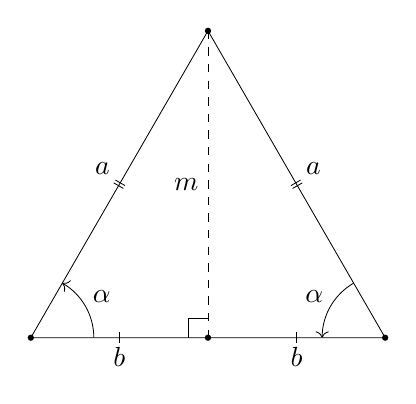
\begin{tikzpicture}[scale=1.0]

% parameters %{{{1

	\def\len{4.5}
	\def\ang{60}

% coordinates %{{{1

	\coordinate (A) at (0,0);
	\coordinate (B) at (0:{2*\len*cos(\ang)});
	\coordinate (C) at (\ang:\len);

	\coordinate (D) at (0:{\len*cos(\ang)});

% points, dots, vertices %{{{1

	\fill (A) circle (0.4mm);
	\fill (B) circle (0.4mm);
	\fill (C) circle (0.4mm);
	\fill (D) circle (0.4mm);

% equilateral triangle %{{{1

	\draw (A) -- (B) -- (C) -- cycle;
	\draw[dashed] (C) -- (D);

% segment labels %{{{1

	\node[above left]  at ($(A)!0.5!(C)$) {$a$};
	\node[above right] at ($(B)!0.5!(C)$) {$a$};

	\node[left]  at ($(C)!0.5!(D)$) {$m$};

	\node[below]  at ($(A)!0.5!(D)$) {$b$};
	\node[below] at ($(D)!0.5!(B)$) {$b$};

% segments, sides marks %{{{1

	\tkzMarkSegments[mark=||, size=2pt](B,C)
	\tkzMarkSegments[mark=||, size=2pt](C,A)

	\tkzMarkSegments[mark=|, size=2pt](A,D)
	\tkzMarkSegments[mark=|, size=2pt](D,B)

% angles labels %{{{1

	\pic[draw, ->, "$\alpha$", angle radius=0.8cm, angle eccentricity=1.3]
	{angle = D--A--C};

	\pic[draw, ->, "$\alpha$", angle radius=0.8cm, angle eccentricity=1.3]
	{angle = C--B--D};

% right angles markers %{{{2

	\pic[draw, angle radius=7pt, angle eccentricity=1.5]
	{right angle = C--D--A};

% closing %{{{1

\end{tikzpicture}
\end{document}
